\chapter{Exploring Activity Recognition in Robogames}

On a~\gls{pirg}, one is often interested in modeling the human player behavior and, from such modeling, program the system to respond properly. Our research began by exploring activity recognition and how that could be incorporated on the design of better~\gls{pirg}'s. 

In the literature, some approaches for activity recognition are based on the analysis of data coming from camera devices. Others, instead, focus on data coming from wearable devices, such as: cellphones, watches and~\gls{imu} -- a specific-purpose device for measuring accelerations and rotation angles. Across years, the type of analysis carried out has pretty much shifted from basic exploratory analysis,~\eg summary statistics, to complex data-based models, such as those from the~\gls{ml} community. The advantage of this is in the fact that~\gls{ml} models often grant better results by the characterization of the hidden structures present in data.

One may spot at least two groups into which to classify works in the area: those performed on an off-line manner and those performed on an on-line one. The first focus on the exploitation of methods for the case were data are first collected, tagged and them processed. The philosophy behind on-line methods, as the name suggests, rely on methodologies that can process the data on the go, providing real-time information about the estimated activity. In all of the vast literature in this field,~\gls{ml}-based approaches rely on some kind of transformation to the data in order to increase recognition results.

In the following, we present how we exploit a simple transformation of the input space targeting the creation of a flexible, generic, and well defined framework for activity recognition in a~\gls{pirg} scenario. To the best of our knowledge, our proposal is the first one to incorporate activity recognition on a~\glsdesc{pirg} involving a human and a mobile robot in a adversarial game setting.

\section{Introduction}

Detailed measurement and classification of an individual's physical  activity is fundamental in order to understand the relationship between physical activity and health but, also, to achieve an enhanced level of interaction between humans and robots. In particular, when considering~\glsdesc{pirg}~\cite{martinoia_physically_2013} -- where the objective is the exploitation of both the real world as environment, and of one or more real, physical, autonomous robots as game opponents or companions of human players -- activity recognition plays a fundamental role to adapt the robot strategy to support the player's entertainment during the game.

Here we propose a model which aims at classifying player's activity in a~\gls{pirg} game using a 3-axis custom accelerometer positioned on the player's chest. We define a set of high level activity classes that are automatically classified relying on a supervised machine learning framework. Our methodology consists of transforming the raw input space into one that is able to capture variance of the signal to emphasize the recognition of the target activities. 

Our main contribution is on the fact that we are able to obtain reasonable results in accuracy by applying a simple transformation. The achieved results are comparable, in terms of accuracy, with sliding window approaches, which makes our method feasible for real applications, but at lower cost regarding data processing. We test out methodology on activity recognition during a real robogame scenario~(see section~\ref{sec:game_environment}). 

The chapter is organized as follows: we first present some related works about activity recognition and classification; In section~\ref{datacollection} we explain how we collected data, while in section~\ref{activityanalysis} we provide the description of the activity model. The results are finally discussed in section~\ref{discussion}.

\section{Related Works}\label{relatedworks}

A number of recent studies have investigated activity recognition using one or more accelerometer placed in different parts of the body. In~\cite{ravi_activity_2005}, a well-cited paper in the activity recognition community, the authors have used a triaxial accelerometer worn near the pelvic region in order to classify eight different daily-life activities: \textit{standing}, \textit{walking}, \textit{running}, \textit{climbing up stairs}, \textit{climbing down stairs}, \textit{sit-ups}, \textit{vacuuming}, and \textit{brushing teeth}.

%The feature extraction from the raw accelerometer data used the \textit{sliding windows} method, a very common stream processing method found in many applications. It consists in the process of making computation on a batch of data, called a windows, that is eventually updated with new incoming data. This update process is referred the``sliding of the windows''. When slided, the windows may retain some of the previous update data points, this is referred to the amount of \textit{overlap} used on the windows. 

The windows size used had 256 data-points with 128 samples overlapping ($50\%$ overlap) between consecutive windows. At a sampling frequency of 50Hz, each window represents data for 5.12 seconds. The ammount of overlap used is justified by the work of~\cite{bao_activity_2004}, where they had demonstrated the feasibility of such overlap. 

%~\cite{mannini2013activity} proposes daily physical activities recognition using a single accelerometer placed at the wrist or ankle. This study uses various combinations of window lengths and feature sets to develop an algorithm with the aim to classify a wide variety of activities into four distinct classes using accelerometer raw data and, also, higher classification accuracies for ankle data w.r.t the wrist data.

%These windows can be either fixed in size by including only the most recent n data points or by showing only the most recent t time units of data (where n and t are constants). While the implementation of this model is very simple, it is prone to errors when choosing a wrong window width. Too narrow windows will produce very accurate representations of the current state, but are heavily affected by noisy data while too wide windows result in more stable yet equally inaccurate results due to the effects of concept drift [2]. Nevertheless, fixed sliding windows can be found in many applications. An example is [7] where they are used to detect regions of abnormal network activity.

%The possibility of performing human activity recognition using raw accelerometer data from smart-phones is also a very common field of study. For example, in~\cite{bayat2014study} an experiment where subjects were requested to perform two different activities has been performed and, given their start and end times, two datasets were considered: one for in-hand phone position and one for in-pocket phone position. This information was then used to label different activities for a supervised learning classification problem. Another similar work was~\cite{anguita2013public}, while in~\cite{su2014activity} a number of applications for such studies are also proposed. %%% EWERTON: This paragraph is strange, it has to give some it doesn't give much information about the studies. The last sentence just mentions papers but doesn't present their goals or methodology. It has to be changed. %%%

Considering a game environment,~\cite{jablonsky_evaluating_2017} investigated sensor placement and modality for activity recognition within the context of children's playground  activities. By mean of parallel sensing, performed using a set of smart-phones, activity dependent data have been generated. The obtained set of data was then used to train decision tree classifiers. This study shows once again that phones placed closer to the core of the body generate better models than phones placed on the  extremities. 

Similarly, in~\cite{alshurafa_designing_2014} a stochastic approximation framework for intensity independent activity recognition based on clustering techniques is proposed. The aim is to enhance and automate the calculation of~\gls{met} and also to improve an exergaming (video games that are also a form of exercise) platform consisting of two main components: an accelerometer-embedded belt and an~\gls{rpg} video game called \textit{FreedroidRPG} that was used as an incentive for the participant to perform physical activity throughout the day. The study shows the ability of the used stochastic approximation framework to extrapolate unknown intensity levels from a few  known ones that can be used to enhance activity recognition.

Several studies in literature also focused on the comparison between multi-sensor versus single-sensor activity detection and also on the optimal body placement of such sensors.

The work of~\cite{gao_evaluation_2014} compared two distinct types of wearable systems: single-sensor wearable systems adopting complex algorithms and multi-sensor systems employing light-weight algorithms. The impact of the sampling rate on the recognition accuracy was then investigated using four classifiers. The experimental results illustrated that the recognition accuracy was steady at 50-Hz and above, and the single sensor system was more sensitive to the sampling rate than the multi-sensor system.

The work of~\cite{trost_machine_2014} is, in turn, focused on making a comparison between the activity recognition rates of an activity classifier trained on acceleration signal collected on the wrist and hip. During the experiments 52 children and adolescents completed 12 activity trials that were categorized into 7 activity classes: \textit{lying down}, \textit{sitting}, \textit{standing}, \textit{walking}, \textit{running}, \textit{basketball}, and \textit{dancing}. As result, the hip model exhibited great classification accuracy for \textit{sitting}, \textit{standing}, \textit{walking}, and \textit{running}; acceptable classification accuracy for \textit{lying down} and \textit{basketball}; and modest accuracy for \textit{dance}. The wrist model, in turn, exhibited excellent classification accuracy for \textit{sitting}, \textit{standing}, and \textit{walking}; acceptable classification accuracy for \textit{basketball}; and modest accuracy for \textit{running}, \textit{lying down} and \textit{dance}.

The present work, follows the line of reasoning present in popular one, such as~\cite{ravi_activity_2005, bao_activity_2004}, where the methodology relies on the use of supervised learning methods, powered by the extraction of discriminative features from a sliding window. However, the use of such method in our application scenario rises same special issues: since the annotated data come from real game interaction between a human and a mobile robot, the activities are not limited in any aspect.

Additionally, when using a traditional sliding window method, special attention has to be made on the choice of window size. This is because while a too narrow window will produce very accurate representations of the current state, it will also be heavily affected by noise. On the other hand, a too wide window results in more stable, yet similarly inaccurate results due to the effects of change in the underlying data~\cite{bifet_learning_2007}. 

Equally concerning, fixed-size windows are likely to ignore differences in the duration of activities. This happens very often in our scenarios where different in-game situations would make the players react differently. For instance, the time the player spends running are a product of multiple factors, including personal motivations and robot state given in-game situation. 

This would demand adaptive strategies for using sliding windows, as suggested by~\cite{noor_adaptive_2016}. However, in this work we follow a different route, by proposing to perform activity recognition by first transforming the data stream input space (acceleration raw data) into a different space that would capture the ``turbulence'' of the signal underlying each activity of interest %(standard deviation of the accelerations along xyz axis) - DAVIDE%. 
The motivation is that a running activity, for example, would be categorized by a different amount of turbulence compared to other activities.
%,such as simply standing or locally moving. - DAVIDE%
\section{The Game Scenario}\label{gamescenario}
In order to test our model, we designed a competitive game, where the human player faces an autonomous robot.

\subsection{The Robotic Platform}\label{roboplat} 
We have adopted a holonomic robot that is free to move in any direction at a maximum speed comparable to that of people in indoor environments (1.4 m/sec).

\begin{figure}[thpb]
    \centering
    \begin{subfigure}[b]{0.3\textwidth}
        \includegraphics[width=3cm,height=3cm]{images/04-activity/mobilerobot.jpeg}
        \caption{the robotic platform.}
    \end{subfigure}
    \begin{subfigure}[b]{0.3\textwidth}
        \includegraphics[width=3cm,height=3cm]{images/04-activity/tubes.jpg}
        \caption{the target tower used in the game (height 110cm).}
    \end{subfigure}
    \caption{}
    \label{fig:robot_tubes}
\end{figure}

The robot body consists of a robust, triangular, omni-directional base 5cm high (with 40 cm in diameter), where motors, batteries and electronics are embedded. On the base, an auxiliary aluminum structure is mounted, having the on-board computer attached laterally and a Kinect sensor on top. In total, the robot is 85cm high (see figure~\ref{fig:robot_tubes}).

\begin{figure}[thpb]
      \centering
      \includegraphics[width=3cm,height=3cm]{images/04-activity/sender.jpg}
      \caption{a) the custom accelerometer device used for human motion extraction based on Arduino Uno and a MPU-6050 breakout board. The data is transmitted to a receiver Arduino via Nrf24l01 radio frequency board.}\label{the_accelerometer}
\end{figure}

\subsection{Game Scenario}
For the present work, the ``playground'' is a rectangular area of 4m$\times$2m where, on each corner, ``towers'' are placed. Each tower is equipped with a button and four LEDs that can be progressively turned on, one by one, by pressing the button on the tower top. Each LED requires the button to be pressed for about 2.5 seconds, meaning that the tower takes about 10 seconds of button push in order to light up all of the four LEDs. Button pressing time is cumulated and can be distributed on different moments. After turning on all LEDs of a particular tower during game play, it is said that the player has captured it.

In order to win, the human player must be able to secure all the existing towers without letting a single one be ruined down by the robot. If, at anytime, a tower falls (because of the robot or player) the game ends and the human player is defeated. 

The robot is a holonomic base (see Figure~\ref{robot}(a)). It is able to move across the entire playground just as the human player and is only constrained by the fact that an already captured tower, or one whose button is currently pressed by the player cannot be teared down. The player can also block the robot path by staying in front of it. Notice that while the player is trying to capture a given tower, the robot can try to put down another one.

The robot must avoid hitting the player at any time during the game. Figure~\ref{robot}(b) presents the towers that were used in the game.

This game is designed so that the robot, given its agility and maximum speed (1.4 m/sec) could always win, but it should show the appropriate and believable behavior to keep the player engaged and interested.
  
\section{Method}

%before the activity analysis section shouldn't we put the data collection section? I think that in this way the explanation keeps its flow and everything it's more readable. Also a reviewer asked us to have a method section with the following subsection: hardware, data collection, feature extraction  -  DAVIDE%  

\subsection{Activity analysis}\label{activityanalysis}

On our game, by using an accelerometer attached to the player, we were mainly interested on identifying activities that would help to describe the player interaction level. For the scope of this work, we aimed at identifying recurrent physical activities that would be useful for achieving that goal. From the collected data (see section~\ref{datacollection}), we were able to identify a few high-level activity types, listed below:

\begin{itemize}
\item  \textbf{running:} describes a running activity. For this paper, multiple styles of running are not considered. For instance, ``fast'' or ``slow'' running are considered as the same.
\item \textbf{walking/dodging:} represents the walking and dodging activity. The latter refers to a sudden quick movement to avoid the robot or to call its attention.
\item  \textbf{locally\_moving:} a player generic motion that is too small to fall into other categories, but not so small to be characterized as inactivity. Robot path-blocking motions also fall into this type of motion.
\item  \textbf{inactive:} motion that are too low in intensity to be characterized as one of the above activities. A crisp threshold is used to delimit this category. 
\end{itemize}

By inspecting the data, we observed that a given player activity would occur in ``bursts'', being followed by a short period of inactivity (or rest), i.e., a short period where the player is not really moving, or the expressed acceleration motion is too small to be related to any fundamental activity of interest.

Resting periods are a common characteristic present in any physical game, both related to the organic human need for resting after an intense physical activity or even during strategic moments of pause. Examples of that can be seen when the player is pushing a button on a tower, or is trying to block the robot's path or is even waiting still for a specific robot position on the environment.

Naturally, on such moments of inactivity, the changes in acceleration are usually small, which produces a relative flatness of the signal (e.g., secs 9-12 and 15-18 on figure~\ref{acc_graph}) and allows for the delimitation of an activity begin/end time.

\begin{figure}[h!]
      \centering
      \includegraphics[width=\linewidth]{images/04-activity/newGraph.eps}
      \caption{Graph of acceleration in x, y and z axis for a game that lasted about 40 seconds.}
      \label{acc_graph}
\end{figure}

One way to describe the activity information carried on by the acceleration patterns is by considering the amount of signal ``turbulence''. As a measure of such turbulence, we rely on the information present on the signal variance. 

For this, we process the incoming data stream by computing the standard deviation of the signal inside a sliding window. This transforms the original input space into a new space where activity information are much easily seen: resulting in the generation of a continuous graph, where pulses refer to a given player's physical activity (see figure~\ref{std_graph}). % Also, in my opinion, this analysis is still representative without being affected by the noise coming from the accelerometer's signal so it's feasible also for cheap devices that cannot guarantee a great measurement accuracy. Do you think is the case to say this? - DAVIDE%

Working this way turns out to be simpler than to perform data annotation by, for instance, using a predefined sliding windows size. In our case, activities, such as ``running'', do not have fixed time duration, which makes the applicability of fixed sliding windows methods not well suitable~\cite{noor_adaptive_2016}.

\begin{figure}[thpb]
      \centering
      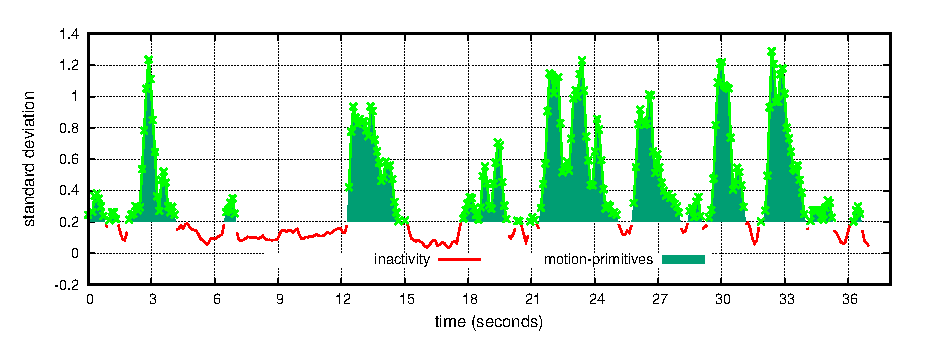
\includegraphics[width=\linewidth]{images/04-activity/newStdGraph.eps}
      \caption{Standard deviation of the acceleration in Figure~\ref{acc_graph}, computed using a sliding window of half a second. The red line portions represent variance values inside the inactivity zone (below a threshold of 0.2). Green areas are referenced as ``motion primitives''.}
      \label{std_graph}
\end{figure}

After performing the mentioned data transformation, we have empirically identified a crisp threshold that would catch irrelevant signal values, thus, we say that any value below that threshold is related to player's inactivity.
% for the sentence above maybe we should say : from data analysis we have EMPIRICALLY determined a crisp threshold (a reviewer asked us to better explain why we choose to set the threshold to 0.2 and the word EMPIRICALLY is enough self explanatory... I think) -  DAVIDE % <-- EWERTON: THE FOLLOWING PARAGRAPH IS ENOUGH FOR THAT!
The inactivity threshold is game-dependent and sensitive to the position of the accelerometer as well. On our experiments, the selection of the inactivity threshold is done manually, via inspection of video recorded during the game.

\begin{figure}[thpb]
    \centering
    \begin{subfigure}[b]{0.3\textwidth}
     	\centering
        \includegraphics[width=3cm,height=3cm]{images/04-activity/enricorun.png}
        \caption{Player performing a running activity.}
	\end{subfigure}
    \begin{subfigure}[b]{0.3\textwidth}
     	\centering
        \includegraphics[width=3cm,height=3cm]{images/04-activity/run1.png}
        \caption{Associated running motion primitive.}
	\end{subfigure}
    \label{running}
\end{figure}

\begin{figure}[thpb]
  \centering
  \begin{subfigure}[b]{0.3\textwidth}
      \includegraphics[width=3cm,height=3cm]{images/04-activity/enricostill.png}
      \caption{Player performing local movements. }
  \end{subfigure}
  \begin{subfigure}[b]{0.3\textwidth}
      \includegraphics[width=3cm,height=3cm]{images/04-activity/still.png}
      \caption{Associated motion primitive.}
  \end{subfigure}
  \label{localmov}
\end{figure}
    
Since any motion information below the threshold is used to determine the ``inactivity'' of the player, we use machine learning-based classification only on each data interval above the threshold. This interval is called a ``motion primitive'' (Figure~\ref{std_graph}). The motion primitives are the data aggregations to which we associate a class label in the annotation procedure. 

Following the classification need, we have extracted the following descriptors from the motion primitives (recall, they refer to standard deviation of the raw values): 

\begin{itemize}
\item \textbf{mean}:  the mean values.
\item \textbf{activity\_time}: the time duration in seconds.
\item \textbf{max\_peaks}:  the max peak.
\item \textbf{number\_of\_peaks}:  the number of peaks.
\item \textbf{mean\_of\_peaks}: the mean of all peaks.
\item \textbf{max-min}: difference between max and min.
\item \textbf{std}: standard deviation.
\item \textbf{mad}: median absolute deviation.
\item \textbf{sma}: signal magnitude area.
\item \textbf{energy}: the signal energy.
\item \textbf{iqr}: interquartile range.
\item \textbf{mean\_over\_max}: mean of peaks divided by the max peak.
\item \textbf{maxInd}: index of the frequency component with largest magnitude.
\item \textbf{meanFreq}:  weighted average of the frequency components to obtain a mean frequency.
\item \textbf{skewness}:  skewness of the motion primitive.
\item \textbf{kurtosis}:  kurtosis of the motion primitive.
\item \textbf{freq-skewness}: skewness of the frequency domain signal.
\item \textbf{freq-kurtosis}: kurtosis of the frequency domain signal.
\item \textbf{pse}: Power spectral entropy.
\item \textbf{rms}: Return the root mean square.
\end{itemize}

%\begin{figure*}[!t]
% ensure that we have normalsize text
%\normalsize
%      \centering
%      {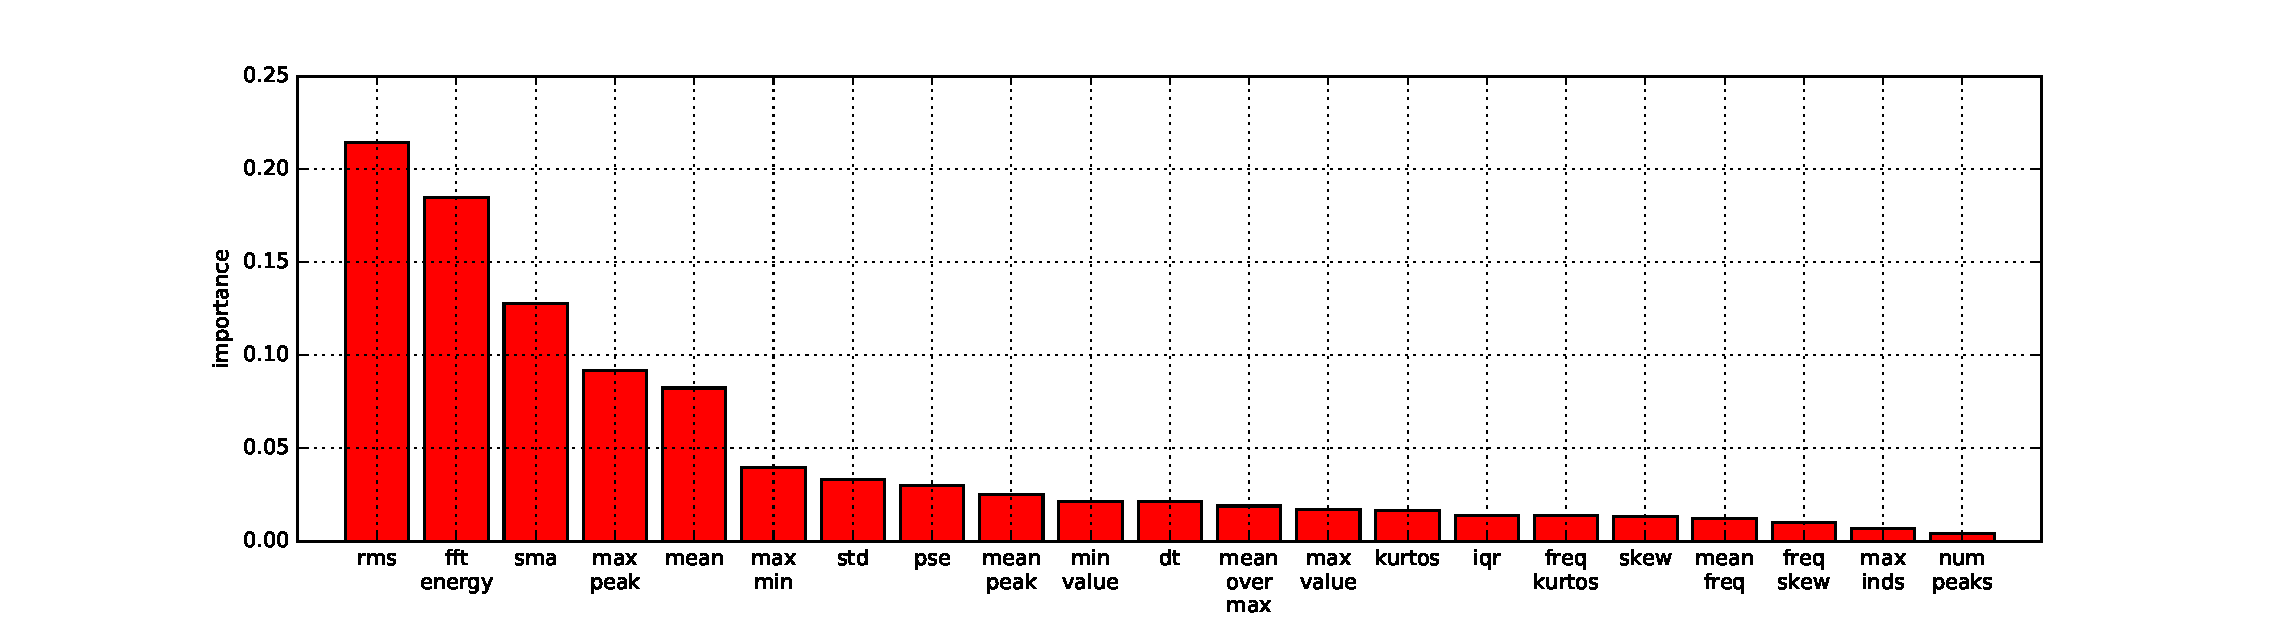
\includegraphics[width=\textwidth]{figures/featureImportance.eps}}
%      \caption{Feature importance computed by a forest of decision trees classifiers.}
%      \label{feature_importance}
%\end{figure*}

Note that, the motion primitives carry sufficient information to distinguish between target physical activities. For example, ``running'' is related to a motion primitive that has a longer duration and a higher amplitude value (see figure~\ref{running}) as opposed to the duration and amplitude values of a player local motion (figure~\ref{localmov}). Following the same argument, a ``walking'' activity has higher amplitude values compared with a local movement. A holistic view of the classification approach is detailed in Figure~\ref{approach}. 

\subsection{Data Collection}\label{datacollection}

When playing the game, we ask the human player to wear a colored robe (see figure~\ref{game}) in order to allow for blob detection and tracking, leading to feature extraction. The visual features extracted in the game are out of the scope of this paper, since we describe only results relying on the accelerometer data.

We have used a custom accelerometer board attached to the player's chest in order to capture a detailed player motion information. The device is based on the InvenSense MPU-6050 3-axis accelerometer board and an Arduino Uno micro-controller. The circuit also contains a Nrf24l01 radio-frequency module that allows the accelerometer data to be sent to the on-board computer. Figure~\ref{the_accelerometer} shows the accelerometer used.

The choice of the accelerometer position was conditioned by the need to minimize the influence of noise from irrelevant player motion.

\begin{figure}[thpb]
      \centering
      {\includegraphics[width=8cm]{images/04-activity/event.jpg}}
      \caption{Human player (in magenta) during the game. The playground configuration consisted of 3 target towers.}
      \label{game}
\end{figure}

For example, because the state of the towers are transmitted to the robot via radio frequency, it is not necessary to identify any related tower activity by means of acceleration patterns. Therefore, having the device placed on the wrist, or other highly movable body-part (as the feet or head) would capture useless acceleration information contributing to a decrease in classification accuracy for the mentioned target motions. 

In terms of collected data, for this work, we considered 29 matches involving 15 male participants of different ages. The age distribution consisted of children (7-10) and adults (26-40). Matches had a minimum time duration of about 40 seconds and a maximum of about 1 minute and 10 seconds. 

The collected data correspond to acceleration values along x, y, and z axis with a sampling frequency of 50Hz, which is five times larger than the frequency considered to be sufficient for detecting daily activities from accelerometer data (10Hz)~\cite{atallah_sensor_2010, ravi_activity_2005, kikhia_analyzing_2014}.

\begin{figure*}[!t]
\normalsize
      \centering
      {\includegraphics[width=\textwidth, height=4cm]{images/04-activity/diagram.png}}
      \caption{Overview of the activity recognition system.}
      \label{approach}
\end{figure*}

\subsection{Classification setup}

As pointed out, for the automatic classification we first build the standard deviation graph from the raw accelerometer data, and then we manually label motion primitives. 

On our experiments, the std graph was generated considering a sliding window 500msec long, resulting on a dataset composed by $367$ motion primitives with $34\%$ labeled as ``locally\_moving''; $25\%$ as ``walking/dodging'' and $41\%$ as ``running''.% and the others? would say a reader - ANDY

Empirically, this time length turned out to be descriptive enough to produce variance intervals that made it possible to distinguish activities. Naturally, the windows size has an impact on the total number of motion primitives generated per game match, as well as on the inactive threshold value. With a windows size of half a second, however, it was possible to capture immediate transition between activities, given that such transition would manifest on higher spikes on variance at the beginning of an activity. For that reason, we kept the mentioned size. 

As argued above, the ``inactive'' type is not considered in the recognition task since it is directly classified by the inactive threshold. From video log inspection, we observed that most of the useless motion would occurs below a threshold of $0.2$. 

Before training classifiers, we performed feature selection by evaluating the importance of the extracted features (see section~\ref{activityanalysis}) using random forest method, composed by 300 decision trees.% (see Figure~\ref{feature_importance}).

\section{Results and discussion}\label{discussion}

We tested different classifiers using 10-fold cross validation in order to have a more descriptive accuracy information. Following common practice, the train-test dataset ratio was defined as 80\% and 20\% respectively.

\begin{table}[h]\footnotesize
  \centering
  \caption{Cross-validation accuracy results for several classification methods using the 5 most significant features.% show in Figure~\ref{feature_importance}.
  }
  \begin{tabular}{| c | c |}
    \hline
  	   \textbf{Method}          & \textbf{Accuracy}\\\hline
       SVM (Linear Kernel)      & 0.80 (+/- 0.08)  \\\hline
       Random Forest            & 0.81 (+/- 0.06)  \\\hline
       Gaussian Naive Bayes     & 0.80 (+/- 0.11)  \\\hline
       Ensemble (Hard voting)   & 0.82 (+/- 0.10)  \\\hline
       AdaBoost                 & 0.65 (+/- 0.40)   \\\hline
  \end{tabular}
  \label{accuracy5best}
\end{table}

\begin{table}[h]\footnotesize
  \centering
  \caption{Classification report for the chosen ensemble method (Random Forest)}
  \begin{tabular}{| c | c | c | c | c |}
    \hline
  	   & precision   & recall & f1-score &  support \\\hline
    LM &      0.88   &  0.91  &    0.89  &      23  \\\hline
    WD &      0.79   &  0.60 &     0.68 &       25  \\\hline
     R &      0.77   &  0.92 &     0.84 &       26  \\\hline
avg/total &   0.81   &  0.81 &     0.80 &       74  \\\hline
  \end{tabular}
  \label{report}
\end{table}

Table~\ref{accuracy5best} presents 10-fold cross validation results using different classifiers on the five most important features, that is: \textit{rms}, \textit{fft\_energy}, \textit{sma}, \textit{max\_peak} and \textit{mean}. 

The ensemble in Table~\ref{accuracy5best} is defined as a majority (Hard) voting approach by the combination of the SVM, Gaussian Naive Bayes and Random Forest. The Adaboost method, in turn, takes a combination of 100 weak classifiers (Decision Trees). All methods were trained by using Python Scikit-learn machine learning library.

Despite the effort, with a confidence interval of 95\% we see that SVM, Random Forest, Gaussian Naive Bayes as well as their ensemble have a similar accuracy result. By considering the variance in their result, we see that Random Forest gives the most stable result. 

Given the 10-fold cross validation results, we decided to use as final method the Random Forest ensemble classifier (10 decision trees). Detailed results for the method are shown in table~\ref{report} and the corresponding confusion matrix and Receiver Operating Characteristic in Figure~\ref{mtx-roc}. The majority of mistakes in the classification correspond to the difficulty in separating ``walking/dodging'' from  a ``running'' activity. 

The justification for this may be on the fact that occasionally the player walks in a fast way what causes an increase in similarity with proper running. This is acceptable given that even for humans it is not straight forward to decide about the boundaries conditions of two different but related activities.

Despite the fact that our method relies on the computation of a fixed slide window when transforming the input data, we see that our method also allows for a small improvement in the annotation procedure. Consider, for example, that we do not have to worry about the effects of overlapping windows. Things like the choice of windowing functions, which are used to mitigate the effects of overlap, are not needed. Also, it allows for a more intuitive way of perceiving what underlying activity has occurred.

We have already conducted experiments on using our method online, and the results have been satisfactory. One drawback, however, is on the possibility of having two different activities associated to the same motion primitive. This is likely to occur when the player rapidly shifts between two activities. For exampl, this happens when the player stops running for a fraction of a second and then immediately starts walking. In that case we see a small decrease in the signal variance that may not be enough to characterize an inactivity period. Note that a value below the inactive threshold is the event that separates motion primitives.

\begin{figure}[thpb]
    \centering
    \begin{subfigure}[b]{\textwidth}
       \centering
       \includegraphics[width=12cm]{images/04-activity/conf_mtx.eps}
       \caption{Confusion matrix for the trained Random Forest ensemble method and the associated.}
	\end{subfigure}
    \begin{subfigure}[b]{\textwidth}
     	\centering
        \includegraphics[width=12cm]{images/04-activity/roc.eps}
        \caption{ROC curve.}
	\end{subfigure}
    \label{running}
\end{figure}

% An example of a floating figure using the graphicx package.
% Note that \label must occur AFTER (or within) \caption.
% For figures, \caption should occur after the \includegraphics.
% Note that IEEEtran v1.7 and later has special internal code that
% is designed to preserve the operation of \label within \caption
% even when the captionsoff option is in effect. However, because
% of issues like this, it may be the safest practice to put all your
% \label just after \caption rather than within \caption{}.
%
% Reminder: the "draftcls" or "draftclsnofoot", not "draft", class
% option should be used if it is desired that the figures are to be
% displayed while in draft mode.
%
%\begin{figure}[!t]
%\centering
%\includegraphics[width=2.5in]{myfigure}
% where an .eps filename suffix will be assumed under latex, 
% and a .pdf suffix will be assumed for pdflatex; or what has been declared
% via \DeclareGraphicsExtensions.
%\caption{Simulation Results}
%\label{fig_sim}
%\end{figure}

% Note that IEEE typically puts floats only at the top, even when this
% results in a large percentage of a column being occupied by floats.


% An example of a double column floating figure using two subfigures.
% (The subfig.sty package must be loaded for this to work.)
% The subfigure \label commands are set within each subfloat command, the
% \label for the overall figure must come after \caption.
% \hfil must be used as a separator to get equal spacing.
% The subfigure.sty package works much the same way, except \subfigure is
% used instead of \subfloat.
%
%\begin{figure*}[!t]
%\centerline{\subfloat[Case I]\includegraphics[width=2.5in]{subfigcase1}%
%\label{fig_first_case}}
%\hfil
%\subfloat[Case II]{\includegraphics[width=2.5in]{subfigcase2}%
%\label{fig_second_case}}}
%\caption{Simulation results}
%\label{fig_sim}
%\end{figure*}
%
% Note that often IEEE papers with subfigures do not employ subfigure
% captions (using the optional argument to \subfloat), but instead will
% reference/describe all of them (a), (b), etc., within the main caption.


% An example of a floating table. Note that, for IEEE style tables, the 
% \caption command should come BEFORE the table. Table text will default to
% \footnotesize as IEEE normally uses this smaller font for tables.
% The \label must come after \caption as always.
%
%\begin{table}[!t]
%% increase table row spacing, adjust to taste
%\renewcommand{\arraystretch}{1.3}
% if using array.sty, it might be a good idea to tweak the value of
% \extrarowheight as needed to properly center the text within the cells
%\caption{An Example of a Table}
%\label{table_example}
%\centering
%% Some packages, such as MDW tools, offer better commands for making tables
%% than the plain LaTeX2e tabular which is used here.
%\begin{tabular}{|c||c|}
%\hline
%One & Two\\
%\hline
%Three & Four\\
%\hline
%\end{tabular}
%\end{table}


% Note that IEEE does not put floats in the very first column - or typically
% anywhere on the first page for that matter. Also, in-text middle ("here")
% positioning is not used. Most IEEE journals/conferences use top floats
% exclusively. Note that, LaTeX2e, unlike IEEE journals/conferences, places
% footnotes above bottom floats. This can be corrected via the \fnbelowfloat
% command of the stfloats package.

\section{Conclusion}
% reviewers said that the paper lacks of novelty. Maybe in the conclusion we should point out again that our methods is designed to be as more general as possible (we don't rely on pre-defined activities, the player is free to move as he want, it works for individuals with very different phisical building etc...). Also some comparison between our results and the one of other studies should be made, I think we should point on the generality of the solution. In general in the conclusion section we should answer to the question "why should I use this method instead of another one???" any idea?? - DAVIDE%
%IDEA 1 - our methods is quite easy to be implemented and does not require a big computational effort, besides in its simplicity is also a powerful and intuitive description method for both type and level of activity with a good level of accuracy (something like this) - DAVIDE%
In this work, we have investigated the recognition of high-level human player activity in a Physically Interactive RobotGame (PIRG) scenario, where a human player faces a mobile robot. We have used the variance in player motion as data instances and primary source of information from where to extract features and then train a machine learning model. 

Physically Interactive RoboGames are a rather new style of game and provide a specific setting from which to study human-robot interaction in situations framed by rules.

In order to design better PIRGs where, for instance, robots can adapt their strategies to support the player entertainment, a player activity model is desired, for which activity recognition is fundamental. We are currently working on the real-time applicability of this method as for the support of methodologies that are capable of quantifying the player engagement by, for instance, analyzing the rate of change in the number of activities performed by the player during the game.